\documentclass[11pt,letterpaper]{article}
\topmargin -.5truein
\textheight 9.0truein
\oddsidemargin 0truein
\evensidemargin 0truein
\textwidth 6.5truein
\setlength{\parskip}{5pt}
\setlength\parindent{0pt}
\usepackage[table]{xcolor}% http://ctan.org/pkg/xcolor
\usepackage{caption}
\usepackage{subcaption}
\usepackage[round]{natbib}
\usepackage{graphicx}
\usepackage{listings}
\usepackage{amsmath}
\usepackage{amssymb}
\usepackage{qtree}
\usepackage{algorithmic}
\usepackage{wrapfig}
\usepackage{tikz}
\usepackage{dsfont}
\usepackage{multirow}
\usepackage[all]{xy}
\usetikzlibrary{arrows,snakes,backgrounds,patterns,matrix,shapes,fit,calc,shadows,plotmarks}



\newcommand{\bs}{\textbackslash}
\renewcommand{\vec}[1]{\mathbf{#1}}

\newcommand{\ngramstart}{\ensuremath{\langle \textsc{s} \rangle}}
\newcommand{\ngramend}{\ensuremath{\langle \textsc{e} \rangle}}
\newcommand{\ngramunk}{\ensuremath{\langle unk \rangle}}

\newcommand{\wcurr}{\ensuremath{w_i}}
\newcommand{\tcurr}{\ensuremath{t_i}}
\newcommand{\tprev}{\ensuremath{t_{i-1}}}

\usepackage{hyperref}
\hypersetup{
    colorlinks,
    citecolor=black,
    filecolor=black,
    linkcolor=black,
    urlcolor=black
}

\title{NLP: Hidden Markov Models}
\author{Dan Garrette\\\small{dhg@cs.utexas.edu}}

\begin{document}
\maketitle



\section{Tagging}

\begin{itemize}
  \item Named entities
  \item Parts of speech
\end{itemize}




\section{Parts of Speech}

Tagsets

\begin{itemize}
  \item Google Universal Tagset, 12: Noun, Verb, Adjective, Adverb, Pronoun, Determiner, Adposition (prepositions and postpositions), Numerals, Conjunctions, Particles, Punctuation, Other
  \item Penn Treebank, 45.  Includes 4 categores of noun, 4 categories of pronoun, and 6 categories of verb.
  \item Brown Corpus, 87
\end{itemize}

Deciding what categories

\begin{itemize}
  \item Auxilliary verbs?  ``I \textit{had} gone''
  \item Numbers as adjectives? ``I saw 4 cars''
  \item Count vs. mass nouns?  ``some apple'' vs. ``two apples'', ``some snow'' vs. ``two snows''
\end{itemize}

Uses

\begin{itemize}
  \item Parsing: determiner and noun should connect first, then to verb
  \item Speech synthesis: OBject (noun) vs. obJECT (verb), CONtent (noun) vs. conTENT (adj)
\end{itemize}

Rule-based

\begin{itemize}
  \item ``if it ends in `-tion' '' $\rightarrow$ Noun
  \item ``if it ends in `-ize' '' $\rightarrow$ Verb
  \item ``if it starts with `re-' '' $\rightarrow$ Verb
  \item ``if it starts with a capital letter'' $\rightarrow$ Proper Noun
  \item ``if it's preceded by `the' '' $\rightarrow$ Noun
  \item ``if it's followed by \textit{'s} '' $\rightarrow$ Noun
  \item ``if it's preceded by an adjective'' $\rightarrow$ Noun
  \item Or just memorize a big list of words and tags?
    \begin{itemize}
      \item Ambiguity?
      \item Picking the most common tag for a word $\rightarrow$ 90\% accuracy (thought state-of-the-art is 97\%)
    \end{itemize}
\end{itemize}

Open vs. Closed

\begin{itemize}
  \item Open class tags: new words are frequently added
    \begin{itemize}
      \item noun, verb, adjective, adverb
      \item ``Twitter'', to ``tweet'', ``twitterish''
    \end{itemize}
  \item Closed class tags: new words are rarely added
    \begin{itemize}
      \item determiner, preposition, pronouns, ...
      \item Don't want to completely close off new words
      \item Maybe \textit{alongside} (preposition) wasn't seen in training, only test
      \item New domains: ``u'' as a pronoun
    \end{itemize}
\end{itemize}

Complexitites:

\begin{itemize}
  \item Ambiguity:
    \begin{itemize}
      \item ``buy a book'' (noun) vs. ``book a flight'' (verb)
      \item ``talk over the deal'' (particle) vs. ``talk over the phone'' (prep)
    \end{itemize}
  \item Phrasal verbs: ``turn down'', ``rule out''
    \begin{itemize}
      \item ``he went on for days''
      \item ``he went on a boat''
    \end{itemize}
\end{itemize}



\section{Hidden Markov Models}


\begin{figure}[p]
\centering
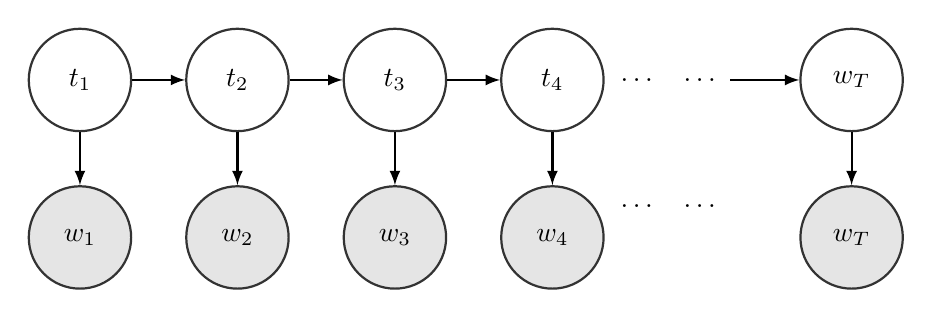
\begin{tikzpicture}
\tikzstyle{main}=[circle, minimum size = 13mm, thick, draw =black!80, node distance = 20mm]
\tikzstyle{obsv}=[main, fill = black!10]
\tikzstyle{hidden}=[node distance = 16mm]
\tikzstyle{connect}=[-latex, thick]
\tikzstyle{box}=[rectangle, draw=black!100]

  \node[main] (t1)                {$t_1$};
  \node[obsv] (w1) [below of =t1] {$w_1$};
  \node[main] (t2) [right of =t1] {$t_2$};
  \node[obsv] (w2) [below of =t2] {$w_2$};
  \node[main] (t3) [right of =t2] {$t_3$};
  \node[obsv] (w3) [below of =t3] {$w_3$};
  \node[main] (t4) [right of =t3] {$t_4$};
  \node[obsv] (w4) [below of =t4] {$w_4$};
  \node[hidden] (tI1) [right of =t4, xshift=-5mm] {$\dots$};
  \node[hidden] (wI1) [below of =tI1] {$\dots$};
  \node[hidden] (tI2) [right of =tI1, xshift=-8mm] {$\dots$};
  \node[hidden] (wI2) [below of =tI2] {$\dots$};
  \node[main] (tT) [right of=tI2, xshift=-1mm] {$w_T$};
  \node[obsv] (wT) [below of=tT] {$w_T$};

  \path (t1) edge [connect] (t2)
        (t2) edge [connect] (t3)
        (t3) edge [connect] (t4)
        (tI2) edge [connect] (tT)
        (t1) edge [connect] (w1)
        (t2) edge [connect] (w2)
        (t3) edge [connect] (w3)
        (t4) edge [connect] (w4)
        (tT) edge [connect] (wT);

\end{tikzpicture}
\caption{Second-order HMM showing conditional dependencies}
\end{figure} 

\begin{figure}[p]
\centering
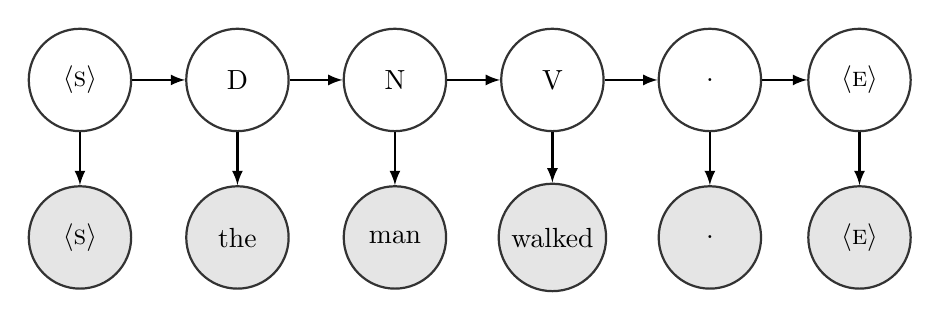
\begin{tikzpicture}
\tikzstyle{main}=[circle, minimum size = 13mm, thick, draw =black!80, node distance = 20mm]
\tikzstyle{obsv}=[main, fill = black!10]
\tikzstyle{hidden}=[node distance = 16mm]
\tikzstyle{connect}=[-latex, thick]
\tikzstyle{box}=[rectangle, draw=black!100]

  \node[main] (t1)                {\ngramstart};
  \node[obsv] (w1) [below of =t1] {\ngramstart};
  \node[main] (t2) [right of =t1] {D};
  \node[obsv] (w2) [below of =t2] {the};
  \node[main] (t3) [right of =t2] {N};
  \node[obsv] (w3) [below of =t3] {man};
  \node[main] (t4) [right of =t3] {V};
  \node[obsv] (w4) [below of =t4] {walked};
  \node[main] (t7) [right of =t4] {.};
  \node[obsv] (w7) [below of =t7] {.};
  \node[main] (tT) [right of =t7, xshift=-1mm] {\ngramend};
  \node[obsv] (wT) [below of =tT] {\ngramend};

  \path (t1) edge [connect] (t2)
        (t2) edge [connect] (t3)
        (t3) edge [connect] (t4)
        (t4) edge [connect] (t7)
        (t7) edge [connect] (tT)

        (t1) edge [connect] (w1)
        (t2) edge [connect] (w2)
        (t3) edge [connect] (w3)
        (t4) edge [connect] (w4)
        (t7) edge [connect] (w7)
        (tT) edge [connect] (wT);

\end{tikzpicture}
\caption{Second-order HMM for the sentence ``the man walks .''}
\end{figure} 



Similar to N-Gram models

\begin{itemize}
  \item Model the text as a \textit{sequence}
    \begin{itemize}
      \item Bad assumption, but less sparse
    \end{itemize}
  \item For ngrams, we modeled the probability of each word conditioned on the previous n-1 words.
  \item Here, we model each \textit{tag} conditioned on previous \textit{tags}
  \item Still uses Markov assumption: only look back a few tags
    \begin{itemize}
      \item Again, bad assumption, but less sparse
    \end{itemize}
  \item Note that we have to condition words on tags because otherwise 
\end{itemize}


~\\ \bs\bs~ Day 2 \\

Derivation

\begin{itemize}
  \item We want the most likely tag sequence for a sequence of words: \vspace{2mm} \\
        $~~~~~~~~~~p(\ngramstart~t_1~t_2~...~t_n~\ngramend \mid \ngramstart~w_1~w_2~...~w_n~\ngramend)$
        \vspace{2mm} \\ Remember that order matters!
  \item For simplicity, we'll write this as $t_1^n = \langle t_1, t_2, ..., t_n \rangle$
  \item So we want  \vspace{2mm} \\
  $~~~~~~~~~~~~~\hat{t}_1^n = \text{argmax}_{t_1^n}~p(\ngramstart~t_1~t_2~...~t_n~\ngramend \mid \ngramstart~w_1~w_2~...~w_n~\ngramend)$ \vspace{2mm} \\ but it's hard to estimate
  \item Like for ngrams, use Bayes rule: 
  \begin{align*}
  \hat{t}_1^n 
  &= \text{argmax}_{t_1^n}~\frac{p(\ngramstart~w_1~w_2~...~w_n~\ngramend \mid \ngramstart~t_1~t_2~...~t_n~\ngramend) \cdot p(\ngramstart~t_1~t_2~...~t_n~\ngramend}{p(\ngramstart~w_1~w_2~...~w_n~\ngramend)} \\
  & = \text{argmax}_{t_1^n}~p(\ngramstart~w_1~w_2~...~w_n~\ngramend \mid \ngramstart~t_1~t_2~...~t_n~\ngramend) \cdot p(\ngramstart~t_1~t_2~...~t_n~\ngramend)
\end{align*}

  \item Two major independence assumptions:
    \begin{itemize}
      \item Like ngrams, assume probability of a sequence is dependent only on recent past:
        \begin{align*}
          p(\ngramstart~t_1~t_2~...~t_n~\ngramend) 
                    &\approx p(t_1 \mid \ngramstart) \cdot 
                              p(t_2 \mid t_1) \cdot 
                              p(t_2 \mid t_2) \cdot 
                              ...  \cdot 
                              p(t_n \mid t_{n-1}) \cdot 
                              p(\ngramend \mid t_n) \\
                    &= \prod_{i=1}^n p(t_i \mid t_{i-1})
        \end{align*}
      \item Also assume word is only dependent on its tag: \vspace{2mm}
        \begin{align*}
          p(\ngramstart~w_1~w_2~...~w_n~\ngramend \mid \ngramstart~t_1~t_2~...~t_n~\ngramend) 
                    &\approx p(w_1 \mid t_1) \cdot 
                             p(w_2 \mid t_2) \cdot 
                             ...  \cdot 
                             p(w_n \mid t_n) \\
                    &= \prod_{i=1}^n p(w_i \mid t_i)
        \end{align*}
      \item Together: 
        \begin{align*}
        \hat{t}_1^n &= \text{argmax}_{t_1^n}~p(\ngramstart~t_1~t_2~...~t_n~\ngramend \mid \ngramstart~w_1~w_2~...~w_n~\ngramend) \\
                    &= \text{argmax}_{t_1^n}~p(\ngramstart~w_1~w_2~...~w_n~\ngramend \mid \ngramstart~t_1~t_2~...~t_n~\ngramend) &&\hspace{-7mm}\cdot p(\ngramstart~t_1~t_2~...~t_n~\ngramend) \\
                    &\approx \text{argmax}_{t_1^n}~\prod_{i=1}^n p(w_i \mid t_i) &&\hspace{-7mm}\cdot \prod_{i=1}^n p(t_i \mid t_{i-1}) \\
                    &= \text{argmax}_{t_1^n}~\prod_{i=1}^n p(w_i \mid t_i) \cdot p(t_i \mid t_{i-1})
        \end{align*}
    \end{itemize}
\end{itemize}


\section{Estimating Parameters: MLE}

Two probability distributions to estimate:

\begin{itemize}
  \item Transitions: probability of a tag, given previous tag, $p(t_i \mid t_{i-1})$
  \item Emissions: probability of a word, given its tag, $p(w_i \mid t_i)$
\end{itemize}

MLE

\begin{itemize}
  \item MLE estimation is just like before (na\"{i}ve Bayes, ngrams, ...): normalized counts
  \item Transitions: $p(t_i \mid t_{i-1}) = \frac{C(t_{i-1}~t_i)}{\sum_x C(t_{i-1}~x)} = \frac{C(t_{i-1}~t_i)}{C(t_{i-1})}$
  \item Emissions: $p(w_i \mid t_i) = \frac{C(t_i,w_i)}{\sum_x C(t_i,x)} = \frac{C(t_i,w_i)}{C(t_i)}$
\end{itemize}

Example dataset (punctuation excluded for simplicity!):
\vspace{-2mm}
\begin{verbatim}
    <S>|<S> the|D man|N walks|V the|D dog|N <E>|<E> 
    <S>|<S> the|D dog|N runs|V <E>|<E> 
    <S>|<S> the|D dog|N walks|V <E>|<E> 
    <S>|<S> the|D man|N walks|V <E>|<E> 
    <S>|<S> a|D man|N saw|V the|D dog|N <E>|<E> 
    <S>|<S> the|D cat|N walks|V <E>|<E> 
\end{verbatim}

Some probabilities:

\begin{itemize}
  \item $p(t_i=\text{V} \mid t_{i-1}=\text{N}) = \frac{C(\text{N V})}{\sum_x C(\text{N } x)} = \frac{6}{8} = 0.75$
  \item $p(t_i=\text{D} \mid t_{i-1}=\text{N}) = \frac{C(\text{N D})}{\sum_x C(\text{N } x)} = \frac{0}{8} = 0.0$
  \\
  \item $p(w_i=\text{dog} \mid t_i=\text{N}) = \frac{C(\text{N,dog})}{\sum_x C(\text{N},x)} = \frac{4}{8} = 0.50$
  \item $p(w_i=\text{the} \mid t_i=\text{N}) = \frac{C(\text{N,the})}{\sum_x C(\text{N},x)} = \frac{0}{8} = 0.0$
\end{itemize}


\section{Add-$\lambda$ Smoothing}

Again, just like before.

\begin{itemize}
  \item Transitions: $p(t_i \mid t_{i-1}) 
             = \frac{C(t_{i-1}~t_i)+\lambda}{\sum_x (C(t_{i-1}~x)+\lambda)} 
             = \frac{C(t_{i-1}~t_i)+\lambda}{(\sum_x C(t_{i-1}~x))+\lambda\cdot|T|} 
             = \frac{C(t_{i-1}~t_i)}{C(t_{i-1})}$
  \item Emissions: $p(w_i \mid t_i) 
             = \frac{C(t_i,w_i)+\lambda}{\sum_x (C(t_i,x)+\lambda)} 
             = \frac{C(t_i,w_i)+\lambda}{(\sum_x C(t_i,x))+\lambda\cdot|V|} 
             = \frac{C(t_i,w_i)}{C(t_i)}$
\end{itemize}

Some probabilities (with $\lambda=2$):

\begin{itemize}
  \item The Vocabulary $V$ is the set of all word types that might be associated with a tag \tcurr:   \vspace{2mm} \\
  $V = \{ a, cat, dog, man, runs, saw, the, walks \}$, ~~$|V|=8$
  \item The Tagset $T$ is the set of all possible tags that could follow a tag \tprev:   \vspace{2mm} \\
        $T = \{ D, N, V, \ngramend \}$, ~~$|T|=4$
  \\
  \item $p(t_i=\text{V} \mid t_{i-1}=\text{N}) 
     = \frac{C(\text{N V})+2}{\sum_{x \in T} (C(\text{N } x)+2)} 
     = \frac{C(\text{N V})+2}{(\sum_{x \in T} C(\text{N } x))+(2 \cdot 4)} 
     = \frac{6+2}{8+8} 
     = \frac{8}{16} = 0.50$
  \item $p(t_i=\text{D} \mid t_{i-1}=\text{N}) 
     = \frac{C(\text{N D})+2}{\sum_{x \in T} (C(\text{N } x)+2)} 
     = \frac{C(\text{N D})+2}{(\sum_{x \in T} C(\text{N } x))+(2 \cdot 4)} 
     = \frac{0+2}{8+8}
     = \frac{2}{16} = 0.125$
  \\
  \item $p(w_i=\text{dog} \mid t_i=\text{N}) 
     = \frac{C(\text{N,dog})}{\sum_{x \in V} (C(\text{N},x)+2)} 
     = \frac{C(\text{N,dog})}{(\sum_{x \in V} C(\text{N},x))+(2 \cdot 8)} 
     = \frac{4+2}{8+16}
     = 0.25$
  \item $p(w_i=\text{the} \mid t_i=\text{N}) 
     = \frac{C(\text{N,the})}{\sum_{x \in V} (C(\text{N},x)+2)} 
     = \frac{C(\text{N,the})}{(\sum_{x \in V} C(\text{N},x))+(2 \cdot 8)} 
     = \frac{0+2}{8+16} 
     = 0.08$
\end{itemize}

Differences:

\begin{itemize}
  \item Two distributions, two kinds of smoothing
  \item Can do add-$\lambda$ for both, but don't need to use same $\lambda$
  \item Can use totally different smoothing for each.
\end{itemize}


\section{One-Count Smoothing}

From Chen and Goodman (1996)

Idea: Smooth conditional distribution by interpolating the MLE with a unigram distribution where the degree of smoothing is proportional to the ``openness'' of a tag.
\begin{align*}
  p(\tcurr \mid \tprev) &= \frac{C(\tprev,\tcurr) + \alpha(\tprev) \cdot p(\tcurr)}{C(\tprev) + \alpha(\tprev)}
  &&\text{where} ~~ \alpha(\tprev) = | \tcurr: C(\tprev,\tcurr) = 1 | \\\\
  p(\wcurr \mid \tcurr) &= \frac{C(\tcurr,\wcurr) + \beta(\tcurr) \cdot p(\wcurr)}{C(\tcurr) + \beta(\tcurr)}
  &&\text{where} ~~ \beta(\tcurr) = | \wcurr: C(\tcurr,\wcurr) = 1 |
\end{align*}

\begin{itemize}
  \item For emissions, if a tag \tcurr\ appears one time with a large number of word types, then we assume that it is very ``open'': there is a large number of words that it has only been seen with once, so the likelihood that it \textit{could have} been seen with some other word, even though it didn't \textit{happen} to be seen with it, is high.
  \item For transitions, the reasoning is the same.  Instead of a tag being associated with a wide variety of words once, it's a wide variety of subsequent tags once.

  \item Note that it is still necessary to smooth the prior distributions $p(\tprev)$ and $p(w_i)$ since if the transition or emission count is zero, we need to ensure that we back off to some non-zero value; add-1 smoothing should be sufficient.  Additionally, It is necessary to add some small amount to $\alpha(\tprev)$ and $\beta(\tcurr)$ in case there are no singletons
\end{itemize}





\newsavebox{\startaltable}
\sbox{\startaltable}{
    \begin{tabular}{l l}
      \hline
      \multicolumn{2}{|c|}{{\cellcolor{gray!40}\ngramstart}} \tabularnewline
      \hline
      \ngramstart & 1.0
    \end{tabular}
}

\newsavebox{\Daltable}
\sbox{\Daltable}{
    \begin{tabular}{l l}
      \hline
      \multicolumn{2}{|c|}{{\cellcolor{gray!40}D}} \tabularnewline
      \hline
      the & 0.47 \tabularnewline
      a   & 0.12 \tabularnewline
      $*$   & 0.06
    \end{tabular}
}

\newsavebox{\Naltable}
\sbox{\Naltable}{
    \begin{tabular}{l l}
      \hline
      \multicolumn{2}{|c|}{{\cellcolor{gray!40}N}} \tabularnewline
      \hline
      man & 0.24 \tabularnewline
      dog & 0.29 \tabularnewline
      cat & 0.12 \tabularnewline
      $*$   & 0.06
    \end{tabular}
}

\newsavebox{\Valtable}
\sbox{\Valtable}{
    \begin{tabular}{l l}
      \hline
      \multicolumn{2}{|c|}{{\cellcolor{gray!40}V}} \tabularnewline
      \hline
      walks  & 0.33 \tabularnewline
      runs   & 0.13 \tabularnewline
      saw    & 0.13 \tabularnewline
      $*$      & 0.07
    \end{tabular}
}

\newsavebox{\ngramendaltable}
\sbox{\ngramendaltable}{
    \begin{tabular}{l l}
      \hline
      \multicolumn{2}{|c|}{{\cellcolor{gray!40}\ngramend}} \tabularnewline
      \hline
      \ngramend & 1.0
    \end{tabular}
}


\begin{figure}[p]
\centering
\begin{tikzpicture}
\tikzstyle{main}=[rectangle, thick, draw =black!80, node distance = 40mm]
\tikzstyle{obsv}=[main, fill = black!10]
\tikzstyle{hidden}=[node distance = 16mm]
\tikzstyle{connect}=[-latex, thick]
\tikzstyle{box}=[rectangle, draw=black!100]

  \node[main] (start) []                         {\usebox{\startaltable}};
  \node[main] (D)     [right of =start]          {\usebox{\Daltable}};
  \node[main] (N)     [right of =D, yshift= 90]  {\usebox{\Naltable}};
  \node[main] (V)     [right of =D, xshift=60, yshift=-90]  {\usebox{\Valtable}};
  \node[main] (end)   [right of =D, xshift=170]   {\usebox{\ngramendaltable}};


  \path (start) edge [connect] node [pos=0.5, above, blue, sloped] {0.78} (D);
  \path (start) edge [connect, bend left=25] node [pos=0.5, above, blue, sloped] {0.11} (N);
  \path (start) edge [connect, bend right=25] node [pos=0.5, below, blue, sloped] {0.11} (V);
  
  \path (D) edge [in=98,out=83,loop] node [pos=0.5, above, blue, sloped] {0.08} (D);
  \path (D) edge [connect, bend left=15] node [pos=0.5, above, blue, sloped] {0.75} (N);
  \path (D) edge [connect, bend right=15] node [pos=0.5, below, blue, sloped] {0.08} (V);
  \path (D) edge [connect, bend left=10] node [pos=0.75, above, blue, sloped] {0.08} (end);

  \path (N) edge [connect, bend left=15, red] node [pos=0.5, above, blue, sloped] {0.08} (D);
  \path (N) edge [in=98,out=83,loop] node [pos=0.5, above, blue, sloped] {0.08} (N);
  \path (N) edge [connect, bend left=15] node [pos=0.5, below, blue, sloped] {0.58} (V);
  \path (N) edge [connect] node [pos=0.5, above, blue, sloped] {0.25} (end);

  \path (V) edge [connect, bend right=15, red] node [pos=0.5, below, blue, sloped] {0.30} (D);
  \path (V) edge [connect, bend left=15, red] node [pos=0.5, below, blue, sloped] {0.10} (N);
  \path (V) edge [in=-98,out=-83,loop] node [pos=0.5, below, blue, sloped] {0.10} (V);
  \path (V) edge [connect] node [pos=0.5, below, blue, sloped] {0.50} (end);
  

\end{tikzpicture}
\caption{Finite state machine of the data with add-1 smoothing.  Missing arrows are assumed to be zero probabilities.  With smoothing, there is an arrow in \textit{both directions} between every pair of tags.}
\end{figure} 


\section{Three Tasks for HMM}

\begin{enumerate}
  \item Likelihood: Given a tagged sequence, determine its likelihood
  \item Decoding: Given an untagged sequence, determine the best tag sequence for it
  \item Learning: Given an untagged sequence, and a set of tags, learn the HMM parameters.
\end{enumerate}



\section{Likelihood of a tagged sentence}

We can compute the likelihood of a particluar sequence of tags for a sentence:

\begin{itemize}
  \item $p(t_1 ... t_n \mid w_1 ... w_n) = \prod_{i=1}^n p(w_i \mid t_i) \cdot p(t_i \mid t_{i-1})$
\end{itemize}


Example: ``the$|$D dog$|$N walks$|$V''
\begin{align*}
  p(t_1 ... t_n \mid w_1 ... w_n) 
    &\approx \prod_{i=1}^n p(w_i \mid t_i) \cdot p(t_i \mid t_{i-1}) \\
    &= p(D \mid \ngramstart) \cdot p(the   \mid D) \cdot
       p(N \mid D)           \cdot p(dog   \mid N) \cdot
       p(V \mid N)           \cdot p(walks \mid V) \cdot
       p(\ngramend \mid V)
\end{align*}

\begin{itemize}
  \item This says that the probability of the tag sequence is the probability of seeing \textit{D} as the first tag, \textit{the} given that the chosen first tag was \textit{D}, \textit{N} given that the previous tag was \textit{D}, \textit{dog} given that the chosen second tag was \textit{N}, etc...
  \item Transition ($p(t_i \mid t_{i-1})$) and emission ($p(w_i \mid t_i)$) values are calculated as above  
\end{itemize}






\section{Decoding}

Tagging a sentence

\begin{itemize}
  \item $\hat{t}_i^n = \text{argmax}_{t_1^n}~p(t_1 ... t_n \mid w_1 ... w_n) \approx \text{argmax}_{t_1^n}~\prod_{i=1}^n p(w_i \mid t_i) \cdot p(t_i \mid t_{i-1})$
  \item For ``the dog walks'', we have to check all combinations: \vspace{2mm} \\
        \ngramstart\ D D D \ngramend  \vspace{2mm} \\
        \ngramstart\ N D D \ngramend  \vspace{2mm} \\
        \ngramstart\ V D D \ngramend  \vspace{2mm} \\
        \ngramstart\ . D D \ngramend  \vspace{2mm} \\
        \ngramstart\ N N D \ngramend  \vspace{2mm} \\
        \ngramstart\ N V D \ngramend  \vspace{2mm} \\
        ...
  \item But this is insane.
\end{itemize}



~\\ \bs\bs~ Day 3 \\

Choosing a tag

\begin{itemize}
  \item Because of our independence assumptions, the probability of each tag is dependent only on its ``Markov blanket'': the previous tag, emitted word, and next tag.  
    \begin{align*} p(t_i \mid \ngramstart~w_1~w_2~...~w_n~\ngramend, \ngramstart~t_1~t_2~...~\mathbf{t_{i-1}~t_{i+1}}~...~t_n~\ngramend)
       &= p(t_i \mid t_{i-1}, w_i, t_{i+1}) \\
       &= p(t_i \mid t_{i-1}) \cdot p(w_i \mid t_i) \cdot p(t_{i+1} \mid t_i)
    \end{align*}
\end{itemize}

Tagging a sentence

\begin{itemize}
  \item We want to make global decisions about tags.
  \item Due to independence, global decisions are made in terms of local decisions
  \item Tagging ``forward'' through the sentence allows us to predict tags based on previous decisions.
  \item But we can't calculate picking a tag changes the probabilities of previous tags.
\end{itemize}

The Viterbi Algorithm

\begin{itemize}
  \item We need to check all possible tag combinations \textit{efficiently}: dynamic programming
  \item We do this by making two passes through the sentence: one forward through the sentence and one backward
  \item The forward pass
    \begin{itemize}
      % \item Compute, for each potential tag value $k$ of \tcurr\ in the sentence, the likelihood of tagging $t_i=k$ given \textit{all possible ways of tagging the $i$-1 previous words}.
      \item Compute, for each potential tag value $k$ of \tcurr\ in the sentence, the highest probability sequence of tags for the previous $i$-1 words and ending with $t_i=k$, given \textit{all possible ways of tagging the $i$-1 previous words}.  This can be simplified with our independence assumptions.
        \begin{align*}
          v_i(k) &= \text{max}_{t_1, ..., t_{i-1}}~p(w_1, ..., w_i, t_1, ..., t_{i-1}, t_i=k) \\
                 &= p(w_i \mid k) \cdot \text{max}_{k' \in T}~v_{i-1}(k') \cdot p(k \mid k')
        \end{align*}
      \item $v_i(k)$ is the probability of the most likely subsequence of tags that accounts for the first $i$ words and ends with tag $t_i = k$.
      % \item Note that this is a \textit{recursive} definitio since the last probability is just the result of this same equation, but for the previous iteration.
      \item So $k$ is the potential tag for the current token $i$
      \item $k'$ is a potential tag for the previous token $i$-1.
      % \item So this equation says that the likelihood of tagging \tcurr\ with some tag $k$ is the probability of emitting the word $w_i$ from $k$, times the sum of the probabilities of any possible tagging of the previous token $i$-1 with some tag $k'$ (given all of \textit{its} possible previous taggings) times the probability of transitioning from $k'$ to $k$.
      \item In terms of the \textbf{Markov blanket}, this covers the connections to the previous tag and the emitted word
    \end{itemize}
  \item The backward pass
    \begin{itemize}
      \item Starting at the end of the sentence with $\hat{t}_N=\ngramend$, use each chosen ``next tag'' along with the viterbi scores (probability of assigning a tag $k$ to $t_i$ given the best possible sequence of tags), to figure out the most likely tag $k$ for $t_i$.
      \item So:
        \[
          \hat{t}_i = \text{argmax}_{k \in T}~v_{i}(k) \cdot P(\hat{t}_{i+1} \mid t_i=k)
        \]
      \item So the chosen tag is one that has a maximally plausible preceding sequence of tags and best connects to the just-selected ``next'' tag.
      \item In terms of the \textbf{Markov blanket}, this adds in the connection to the next tag (since it has now been decided) to the forward probability which is made up of connections to the previous tag and the emitted word
    \end{itemize}
\end{itemize}




\begin{figure}[p]
\centering
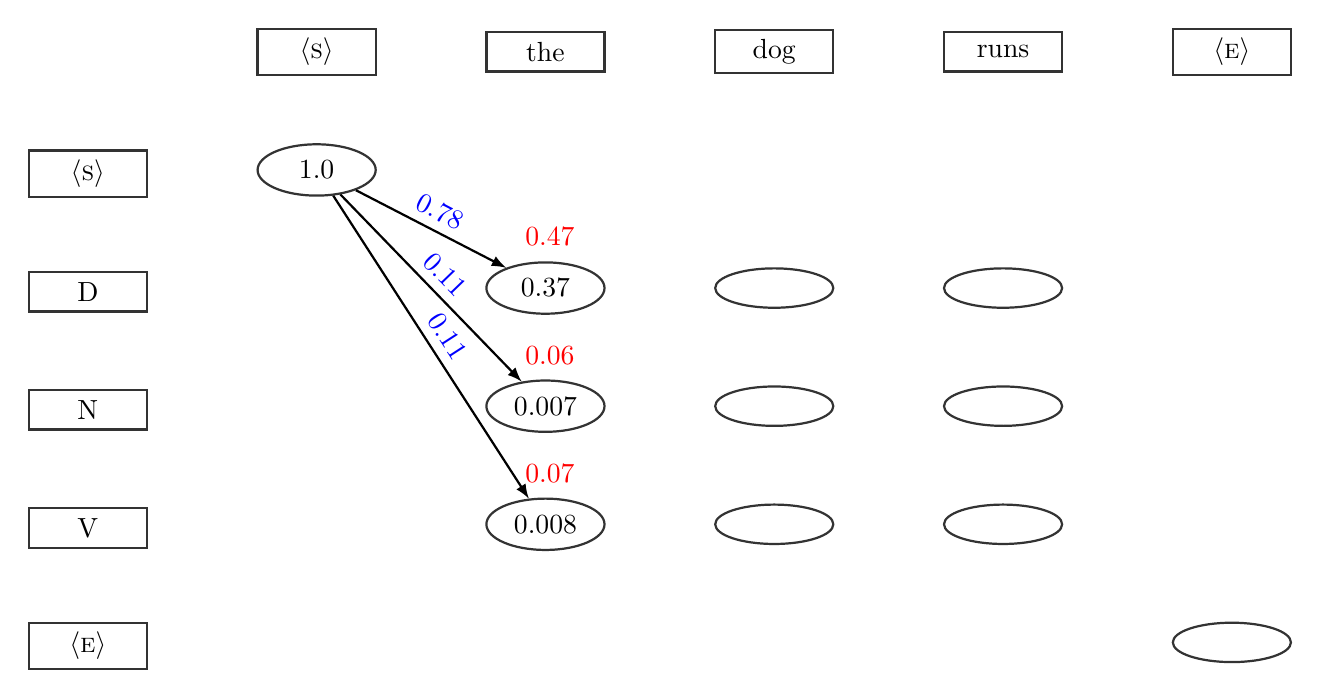
\begin{tikzpicture}
\tikzstyle{main}=[ellipse, thick, draw =black!80, node distance = 15mm, minimum height = 5mm, minimum width = 15mm]
\tikzstyle{rect}=[main, rectangle]
\tikzstyle{obsv}=[main, fill = black!10]
\tikzstyle{hidden}=[main, draw=white]
\tikzstyle{connect}=[-latex, thick]
\tikzstyle{box}=[rectangle, draw=black!100]

  
  \node[rect] (start) []                {\ngramstart};
  \node[rect] (D)     [below of =start] {D};
  \node[rect] (N)     [below of =D]     {N};
  \node[rect] (V)     [below of =N]     {V};
  \node[rect] (end)   [below of =V]     {\ngramend};

  \node[rect] (starttok) [right of =start,    xshift=40, yshift=44]   {\ngramstart};
  \node[rect] (the)      [right of =starttok, xshift=40]              {the};
  \node[rect] (dog)      [right of =the,      xshift=40]              {dog};
  \node[rect] (runs)     [right of =dog,      xshift=40]              {runs};
  \node[rect] (endtok)   [right of =runs,     xshift=40]              {\ngramend};

  \node[main] (startstart)  [below of =starttok]  {1.0};

  \node[hidden] (startthe)  [below of =the]       {};
  \node[main] (Dthe)        [below of =startthe]  {0.37};
  \node[draw, draw=white] at ([shift={(85:0.65)}]Dthe) {\color{red}0.47};
  \node[main] (Nthe)        [below of =Dthe]      {0.007};
  \node[draw, draw=white] at ([shift={(85:0.65)}]Nthe) {\color{red}0.06};
  \node[main] (Vthe)        [below of =Nthe]      {0.008};
  \node[draw, draw=white] at ([shift={(85:0.65)}]Vthe) {\color{red}0.07};
  \node[hidden] (endthe)    [below of =Vthe]      {};

  \node[hidden] (startdog)  [below of =dog]       {};
  \node[main] (Ddog)        [below of =startdog]  {};
  \node[main] (Ndog)        [below of =Ddog]      {};
  \node[main] (Vdog)        [below of =Ndog]      {};
  \node[hidden] (enddog)    [below of =Vdog]      {};

  \node[hidden] (startruns) [below of =runs]      {};
  \node[main] (Druns)       [below of =startruns] {};
  \node[main] (Nruns)       [below of =Druns]     {};
  \node[main] (Vruns)       [below of =Nruns]     {};
  \node[hidden] (endruns)   [below of =Vruns]     {};

  \node[hidden] (startend)  [below of =endtok]    {};
  \node[hidden] (Dend)      [below of =startend]  {};
  \node[hidden] (Nend)      [below of =Dend]      {};
  \node[hidden] (Vend)      [below of =Nend]      {};
  \node[main]   (endend)    [below of =Vend]      {};


  
  \path (startstart) edge [connect] node [pos=0.5, above, blue, sloped] {0.78} (Dthe);
  \path (startstart) edge [connect] node [pos=0.5, above, blue, sloped] {0.11} (Nthe);
  \path (startstart) edge [connect] node [pos=0.5, above, blue, sloped] {0.11} (Vthe);
  

\end{tikzpicture}
\caption{Viterbi Algorithm: 
  Calculating $v_1(D)$, $v_1(N)$, and $v_1(V)$.  Since \ngramstart\ is only choice for the previous tag, each score $v_1(k)$ is calculated as $p(\text{the} \mid k) \cdot v_0(\ngramstart) \cdot p(k \mid \ngramstart)$.  So, for example, \\\\ ~~~~~~ $v_1(D) = p(\text{the} \mid D) \cdot v_0(\ngramstart) \cdot p(D \mid \ngramstart) = 0.47 \cdot 1.0 \cdot 0.78 = 0.37$
}
\end{figure} 





\begin{figure}[p]
\centering
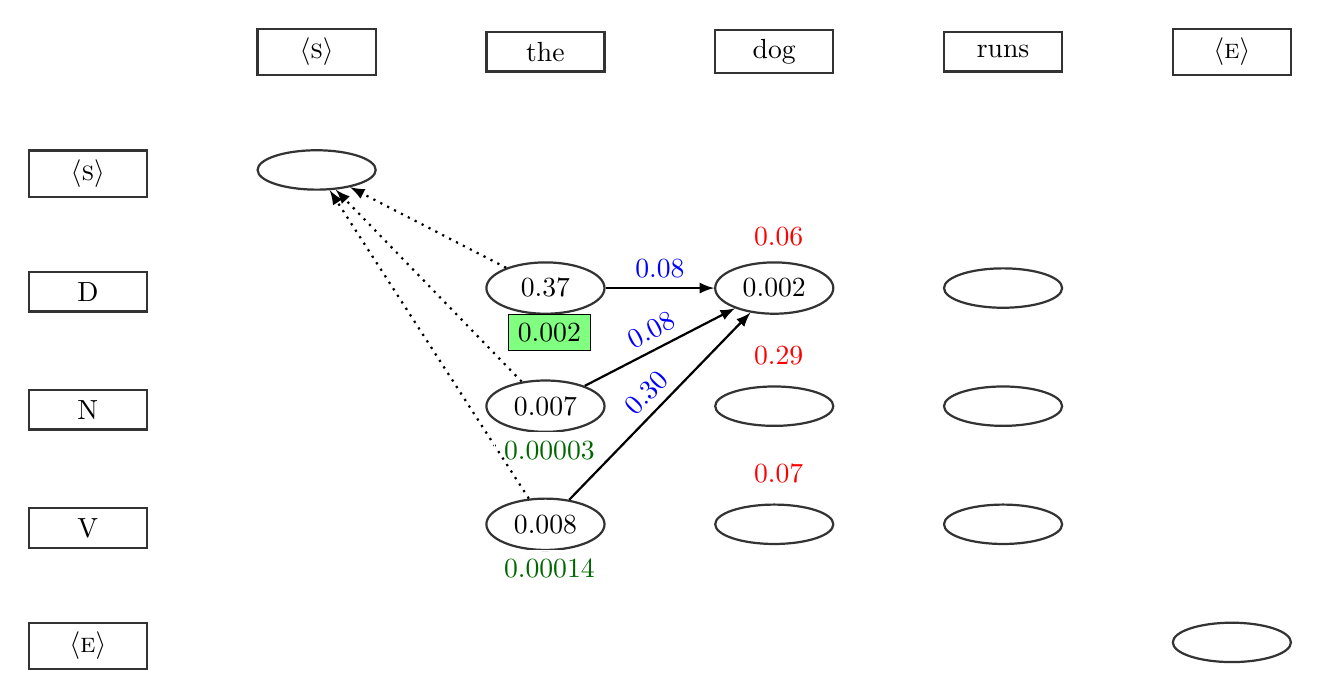
\begin{tikzpicture}
\tikzstyle{main}=[ellipse, thick, draw =black!80, node distance = 15mm, minimum height = 5mm, minimum width = 15mm]
\tikzstyle{rect}=[main, rectangle]
\tikzstyle{obsv}=[main, fill = black!10]
\tikzstyle{hidden}=[main, draw=white]
\tikzstyle{connect}=[-latex, thick]
\tikzstyle{box}=[rectangle, draw=black!100]

  
  \node[rect] (start) []                {\ngramstart};
  \node[rect] (D)     [below of =start] {D};
  \node[rect] (N)     [below of =D]     {N};
  \node[rect] (V)     [below of =N]     {V};
  \node[rect] (end)   [below of =V]     {\ngramend};

  \node[rect] (starttok) [right of =start,    xshift=40, yshift=44]   {\ngramstart};
  \node[rect] (the)      [right of =starttok, xshift=40]              {the};
  \node[rect] (dog)      [right of =the,      xshift=40]              {dog};
  \node[rect] (runs)     [right of =dog,      xshift=40]              {runs};
  \node[rect] (endtok)   [right of =runs,     xshift=40]              {\ngramend};

  \node[main] (startstart)  [below of =starttok]  {};

  \node[hidden] (startthe)  [below of =the]       {};
  \node[main] (Dthe)        [below of =startthe]  {0.37};
  \node[main] (Nthe)        [below of =Dthe]      {0.007};
  \node[main] (Vthe)        [below of =Nthe]      {0.008};
  \node[hidden] (endthe)    [below of =Vthe]      {};

  \node[hidden] (startdog)  [below of =dog]       {};
  \node[main] (Ddog)        [below of =startdog]  {0.002};
  \node[draw, draw=white] at ([shift={(85:0.65)}]Ddog) {\color{red}0.06};
  \node[main] (Ndog)        [below of =Ddog]      {};
  \node[draw, draw=white] at ([shift={(85:0.65)}]Ndog) {\color{red}0.29};
  \node[main] (Vdog)        [below of =Ndog]      {};
  \node[draw, draw=white] at ([shift={(85:0.65)}]Vdog) {\color{red}0.07};
  \node[hidden] (enddog)    [below of =Vdog]      {};

  \node[hidden] (startruns) [below of =runs]      {};
  \node[main] (Druns)       [below of =startruns] {};
  \node[main] (Nruns)       [below of =Druns]     {};
  \node[main] (Vruns)       [below of =Nruns]     {};
  \node[hidden] (endruns)   [below of =Vruns]     {};

  \node[hidden] (startend)  [below of =endtok]    {};
  \node[hidden] (Dend)      [below of =startend]  {};
  \node[hidden] (Nend)      [below of =Dend]      {};
  \node[hidden] (Vend)      [below of =Nend]      {};
  \node[main]   (endend)    [below of =Vend]      {};


  
  \path (Dthe) edge [connect, dotted] (startstart);
  \path (Nthe) edge [connect, dotted] (startstart);
  \path (Vthe) edge [connect, dotted] (startstart);
  
  \node[draw, fill=white!50!green] at ([shift={(95:-0.57)}]Dthe) {0.002};
  \node[draw, draw=white] at ([shift={(95:-0.57)}]Nthe) {\color{black!60!green}0.00003};
  \node[draw, draw=white] at ([shift={(95:-0.57)}]Vthe) {\color{black!60!green}0.00014};

  \path (Dthe) edge [connect] node [pos=0.5, above, blue, sloped] {0.08} (Ddog);
  \path (Nthe) edge [connect] node [pos=0.5, above, blue, sloped] {0.08} (Ddog);
  \path (Vthe) edge [connect] node [pos=0.5, above, blue, sloped] {0.30} (Ddog);
  

\end{tikzpicture}
\caption{Viterbi Algorithm: 
  Find the maximum probability of all possible tag sequences leading to dog$|$D at token $i$.  We do so by finding the best previous tag for getting there, given all possible ways of getting to the previous token.  Since each viterbi score $v_1(k)$ stores the highest probability path for getting to $t_1=k$, all we need to do is find the best way of getting to $t_2=D$ given all the best ways of getting to each possible tag for the previous token, and the probabilities of getting from each possible previous tag to $k$. For example:\\\\
  ~~~~ $v_2(D) = p(\text{dog}|D) \cdot \text{max}(v_1(D) \cdot p(D|D), v_1(N) \cdot p(D|N), v_1(V) \cdot p(D|V)) \\
  ~~~~ ~~~~ ~ = 0.06 \cdot \text{max}(0.37 \cdot 0.08, 0.007 \cdot 0.08, 0.008 \cdot 0.30) \\
  ~~~~ ~~~~ ~ = 0.06 \cdot \text{max}(0.03, 0.0006, 0.002) \\
  ~~~~ ~~~~ ~ = 0.06 \cdot 0.03 \\
  ~~~~ ~~~~ ~ = 0.002$ \\\\
  $t_1=D$ turns out to be the best previous tag for getting to $t_2=D$, so $t_1=D$ is remembered (with a dotted arrow) as the best way to get to $t_2=D$.
}
\end{figure} 





\begin{figure}[p]
\centering
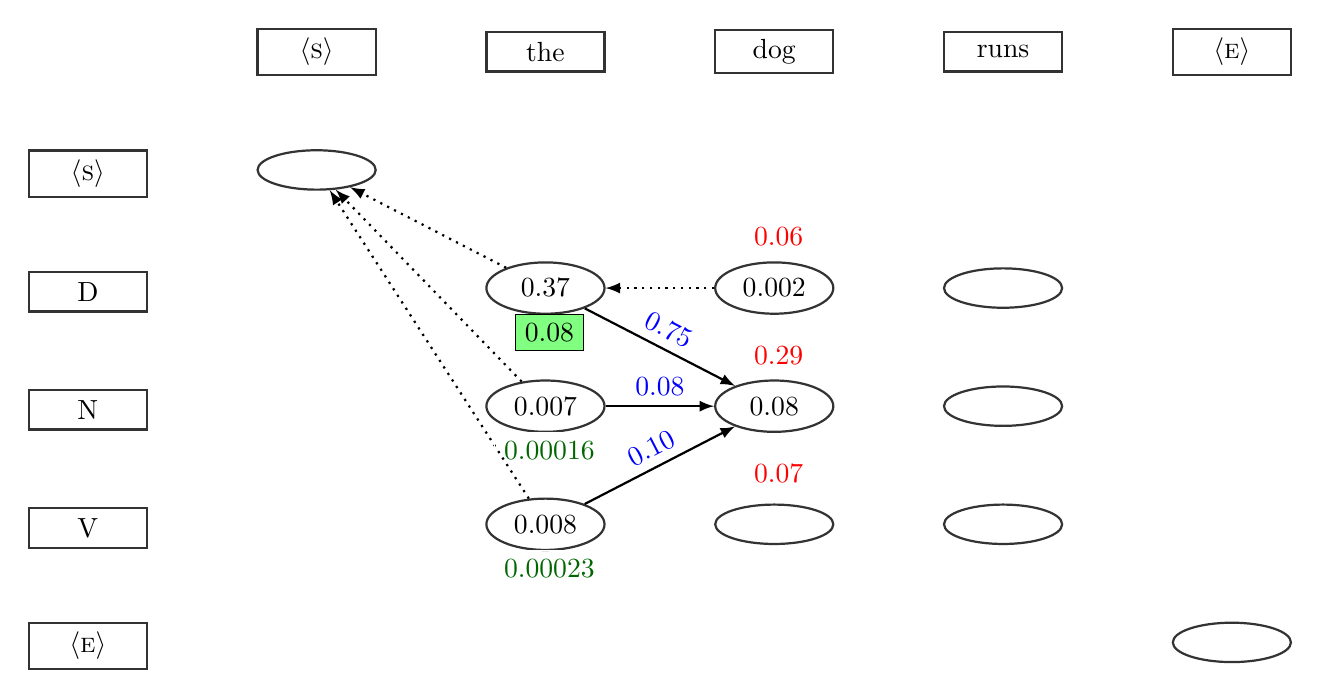
\begin{tikzpicture}
\tikzstyle{main}=[ellipse, thick, draw =black!80, node distance = 15mm, minimum height = 5mm, minimum width = 15mm]
\tikzstyle{rect}=[main, rectangle]
\tikzstyle{obsv}=[main, fill = black!10]
\tikzstyle{hidden}=[main, draw=white]
\tikzstyle{connect}=[-latex, thick]
\tikzstyle{box}=[rectangle, draw=black!100]

  
  \node[rect] (start) []                {\ngramstart};
  \node[rect] (D)     [below of =start] {D};
  \node[rect] (N)     [below of =D]     {N};
  \node[rect] (V)     [below of =N]     {V};
  \node[rect] (end)   [below of =V]     {\ngramend};

  \node[rect] (starttok) [right of =start,    xshift=40, yshift=44]   {\ngramstart};
  \node[rect] (the)      [right of =starttok, xshift=40]              {the};
  \node[rect] (dog)      [right of =the,      xshift=40]              {dog};
  \node[rect] (runs)     [right of =dog,      xshift=40]              {runs};
  \node[rect] (endtok)   [right of =runs,     xshift=40]              {\ngramend};

  \node[main] (startstart)  [below of =starttok]  {};

  \node[hidden] (startthe)  [below of =the]       {};
  \node[main] (Dthe)        [below of =startthe]  {0.37};
  \node[main] (Nthe)        [below of =Dthe]      {0.007};
  \node[main] (Vthe)        [below of =Nthe]      {0.008};
  \node[hidden] (endthe)    [below of =Vthe]      {};

  \node[hidden] (startdog)  [below of =dog]       {};
  \node[main] (Ddog)        [below of =startdog]  {0.002};
  \node[draw, draw=white] at ([shift={(85:0.65)}]Ddog) {\color{red}0.06};
  \node[main] (Ndog)        [below of =Ddog]      {0.08};
  \node[draw, draw=white] at ([shift={(85:0.65)}]Ndog) {\color{red}0.29};
  \node[main] (Vdog)        [below of =Ndog]      {};
  \node[draw, draw=white] at ([shift={(85:0.65)}]Vdog) {\color{red}0.07};
  \node[hidden] (enddog)    [below of =Vdog]      {};

  \node[hidden] (startruns) [below of =runs]      {};
  \node[main] (Druns)       [below of =startruns] {};
  \node[main] (Nruns)       [below of =Druns]     {};
  \node[main] (Vruns)       [below of =Nruns]     {};
  \node[hidden] (endruns)   [below of =Vruns]     {};

  \node[hidden] (startend)  [below of =endtok]    {};
  \node[hidden] (Dend)      [below of =startend]  {};
  \node[hidden] (Nend)      [below of =Dend]      {};
  \node[hidden] (Vend)      [below of =Nend]      {};
  \node[main]   (endend)    [below of =Vend]      {};


  
  \path (Dthe) edge [connect, dotted] (startstart);
  \path (Nthe) edge [connect, dotted] (startstart);
  \path (Vthe) edge [connect, dotted] (startstart);
  \path (Ddog) edge [connect, dotted] (Dthe);


  \node[draw, fill=white!50!green] at ([shift={(95:-0.57)}]Dthe) {0.08};
  \node[draw, draw=white] at ([shift={(95:-0.57)}]Nthe) {\color{black!60!green}0.00016};
  \node[draw, draw=white] at ([shift={(95:-0.57)}]Vthe) {\color{black!60!green}0.00023};

  \path (Dthe) edge [connect] node [pos=0.5, above, blue, sloped] {0.75} (Ndog);
  \path (Nthe) edge [connect] node [pos=0.5, above, blue, sloped] {0.08} (Ndog);
  \path (Vthe) edge [connect] node [pos=0.5, above, blue, sloped] {0.10} (Ndog);
  

\end{tikzpicture}
\caption{Viterbi Algorithm: Calculate $v_2(N)$ and find the best path to it, which turns out to be the path ending with $t_1=D$.}
\end{figure} 





\begin{figure}[p]
\centering
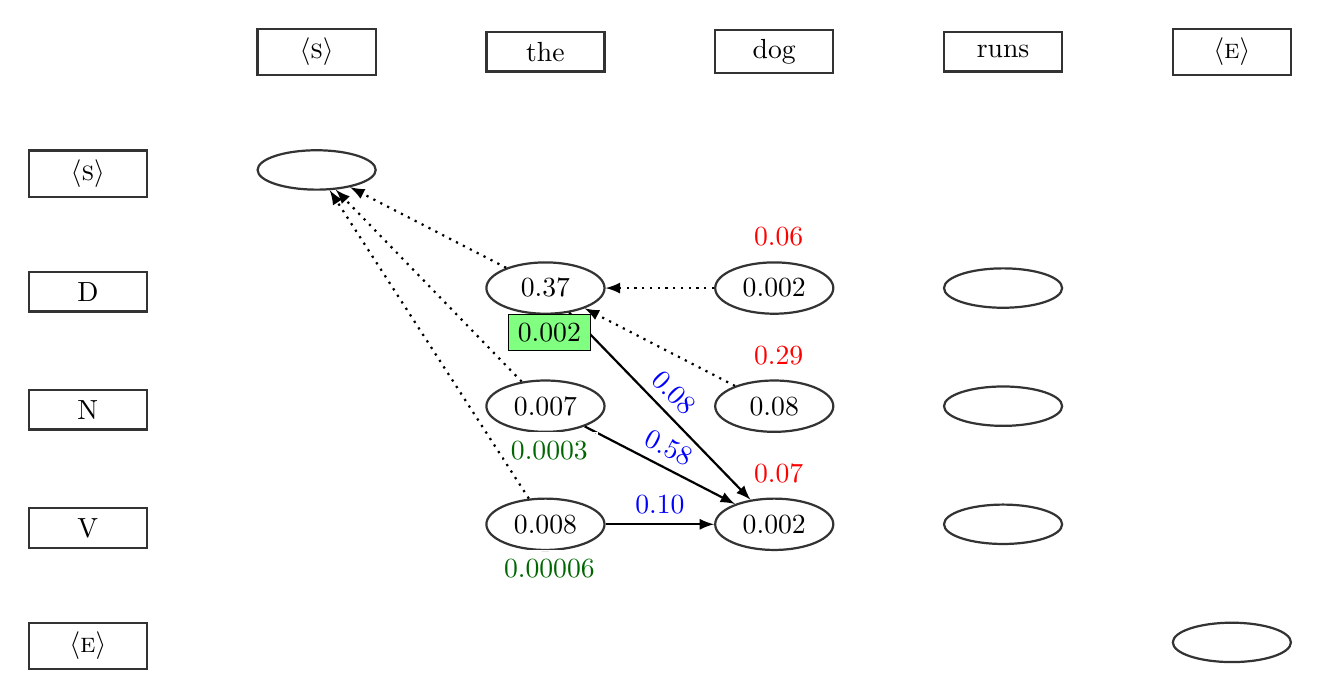
\begin{tikzpicture}
\tikzstyle{main}=[ellipse, thick, draw =black!80, node distance = 15mm, minimum height = 5mm, minimum width = 15mm]
\tikzstyle{rect}=[main, rectangle]
\tikzstyle{obsv}=[main, fill = black!10]
\tikzstyle{hidden}=[main, draw=white]
\tikzstyle{connect}=[-latex, thick]
\tikzstyle{box}=[rectangle, draw=black!100]

  
  \node[rect] (start) []                {\ngramstart};
  \node[rect] (D)     [below of =start] {D};
  \node[rect] (N)     [below of =D]     {N};
  \node[rect] (V)     [below of =N]     {V};
  \node[rect] (end)   [below of =V]     {\ngramend};

  \node[rect] (starttok) [right of =start,    xshift=40, yshift=44]   {\ngramstart};
  \node[rect] (the)      [right of =starttok, xshift=40]              {the};
  \node[rect] (dog)      [right of =the,      xshift=40]              {dog};
  \node[rect] (runs)     [right of =dog,      xshift=40]              {runs};
  \node[rect] (endtok)   [right of =runs,     xshift=40]              {\ngramend};

  \node[main] (startstart)  [below of =starttok]  {};

  \node[hidden] (startthe)  [below of =the]       {};
  \node[main] (Dthe)        [below of =startthe]  {0.37};
  \node[main] (Nthe)        [below of =Dthe]      {0.007};
  \node[main] (Vthe)        [below of =Nthe]      {0.008};
  \node[hidden] (endthe)    [below of =Vthe]      {};

  \node[hidden] (startdog)  [below of =dog]       {};
  \node[main] (Ddog)        [below of =startdog]  {0.002};
  \node[draw, draw=white] at ([shift={(85:0.65)}]Ddog) {\color{red}0.06};
  \node[main] (Ndog)        [below of =Ddog]      {0.08};
  \node[draw, draw=white] at ([shift={(85:0.65)}]Ndog) {\color{red}0.29};
  \node[main] (Vdog)        [below of =Ndog]      {0.002};
  \node[draw, draw=white] at ([shift={(85:0.65)}]Vdog) {\color{red}0.07};
  \node[hidden] (enddog)    [below of =Vdog]      {};

  \node[hidden] (startruns) [below of =runs]      {};
  \node[main] (Druns)       [below of =startruns] {};
  \node[main] (Nruns)       [below of =Druns]     {};
  \node[main] (Vruns)       [below of =Nruns]     {};
  \node[hidden] (endruns)   [below of =Vruns]     {};

  \node[hidden] (startend)  [below of =endtok]    {};
  \node[hidden] (Dend)      [below of =startend]  {};
  \node[hidden] (Nend)      [below of =Dend]      {};
  \node[hidden] (Vend)      [below of =Nend]      {};
  \node[main]   (endend)    [below of =Vend]      {};


  
  \path (Dthe) edge [connect, dotted] (startstart);
  \path (Nthe) edge [connect, dotted] (startstart);
  \path (Vthe) edge [connect, dotted] (startstart);
  \path (Ddog) edge [connect, dotted] (Dthe);
  \path (Ndog) edge [connect, dotted] (Dthe);


  \path (Dthe) edge [connect] node [pos=0.5, above, blue, sloped] {0.08} (Vdog);
  \path (Nthe) edge [connect] node [pos=0.5, above, blue, sloped] {0.58} (Vdog);
  \path (Vthe) edge [connect] node [pos=0.5, above, blue, sloped] {0.10} (Vdog);
  
  \node[draw, fill=white!50!green] at ([shift={(95:-0.57)}]Dthe) {0.002};
  \node[draw, draw=white] at ([shift={(95:-0.57)}]Nthe) {\color{black!60!green}0.0003};
  \node[draw, draw=white] at ([shift={(95:-0.57)}]Vthe) {\color{black!60!green}0.00006};


\end{tikzpicture}
\caption{Viterbi Algorithm: Calculate $v_2(V)$ and find the best path to it, which turns out to be the path ending with $t_1=D$}
\end{figure} 






\begin{figure}[p]
\centering
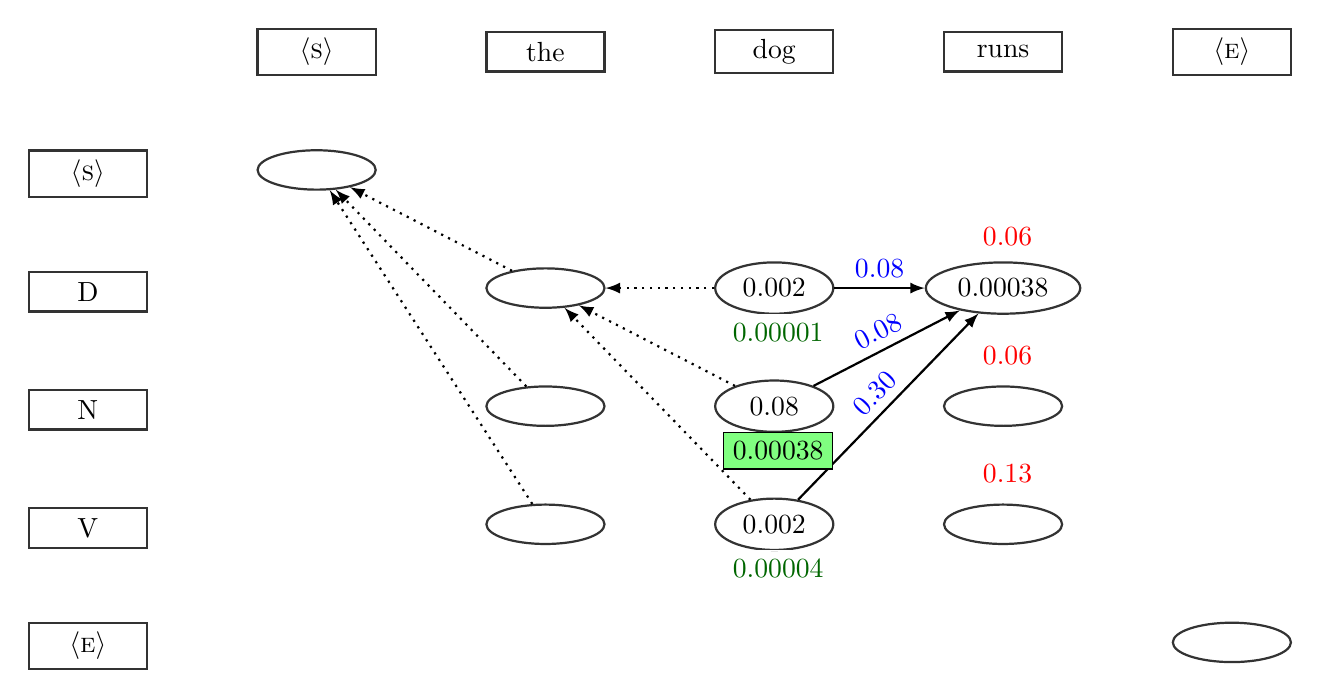
\begin{tikzpicture}
\tikzstyle{main}=[ellipse, thick, draw =black!80, node distance = 15mm, minimum height = 5mm, minimum width = 15mm]
\tikzstyle{rect}=[main, rectangle]
\tikzstyle{obsv}=[main, fill = black!10]
\tikzstyle{hidden}=[main, draw=white]
\tikzstyle{connect}=[-latex, thick]
\tikzstyle{box}=[rectangle, draw=black!100]

  
  \node[rect] (start) []                {\ngramstart};
  \node[rect] (D)     [below of =start] {D};
  \node[rect] (N)     [below of =D]     {N};
  \node[rect] (V)     [below of =N]     {V};
  \node[rect] (end)   [below of =V]     {\ngramend};

  \node[rect] (starttok) [right of =start,    xshift=40, yshift=44]   {\ngramstart};
  \node[rect] (the)      [right of =starttok, xshift=40]              {the};
  \node[rect] (dog)      [right of =the,      xshift=40]              {dog};
  \node[rect] (runs)     [right of =dog,      xshift=40]              {runs};
  \node[rect] (endtok)   [right of =runs,     xshift=40]              {\ngramend};

  \node[main] (startstart)  [below of =starttok]  {};

  \node[hidden] (startthe)  [below of =the]       {};
  \node[main] (Dthe)        [below of =startthe]  {};
  \node[main] (Nthe)        [below of =Dthe]      {};
  \node[main] (Vthe)        [below of =Nthe]      {};
  \node[hidden] (endthe)    [below of =Vthe]      {};

  \node[hidden] (startdog)  [below of =dog]       {};
  \node[main] (Ddog)        [below of =startdog]  {0.002};
  \node[main] (Ndog)        [below of =Ddog]      {0.08};
  \node[main] (Vdog)        [below of =Ndog]      {0.002};
  \node[hidden] (enddog)    [below of =Vdog]      {};

  \node[hidden] (startruns) [below of =runs]      {};
  \node[main] (Druns)       [below of =startruns] {0.00038};
  \node[draw, draw=white] at ([shift={(85:0.65)}]Druns) {\color{red}0.06};
  \node[main] (Nruns)       [below of =Druns]     {};
  \node[draw, draw=white] at ([shift={(85:0.65)}]Nruns) {\color{red}0.06};
  \node[main] (Vruns)       [below of =Nruns]     {};
  \node[draw, draw=white] at ([shift={(85:0.65)}]Vruns) {\color{red}0.13};
  \node[hidden] (endruns)   [below of =Vruns]     {};

  \node[hidden] (startend)  [below of =endtok]    {};
  \node[hidden] (Dend)      [below of =startend]  {};
  \node[hidden] (Nend)      [below of =Dend]      {};
  \node[hidden] (Vend)      [below of =Nend]      {};
  \node[main]   (endend)    [below of =Vend]      {};


  
  \path (Dthe) edge [connect, dotted] (startstart);
  \path (Nthe) edge [connect, dotted] (startstart);
  \path (Vthe) edge [connect, dotted] (startstart);
  \path (Ddog) edge [connect, dotted] (Dthe);
  \path (Ndog) edge [connect, dotted] (Dthe);
  \path (Vdog) edge [connect, dotted] (Dthe);

  \path (Ddog) edge [connect] node [pos=0.5, above, blue, sloped] {0.08} (Druns);
  \path (Ndog) edge [connect] node [pos=0.5, above, blue, sloped] {0.08} (Druns);
  \path (Vdog) edge [connect] node [pos=0.5, above, blue, sloped] {0.30} (Druns);
  
  \node[draw, draw=white] at ([shift={(95:-0.57)}]Ddog) {\color{black!60!green}0.00001};
  \node[draw, fill=white!50!green] at ([shift={(95:-0.57)}]Ndog) {0.00038};
  \node[draw, draw=white] at ([shift={(95:-0.57)}]Vdog) {\color{black!60!green}0.00004};

  

\end{tikzpicture}
\caption{Viterbi Algorithm: Calculate $v_3(D)$ and find the best path to it, which turns out to be the path ending with $t_2=N$}
\end{figure} 





\begin{figure}[p]
\centering
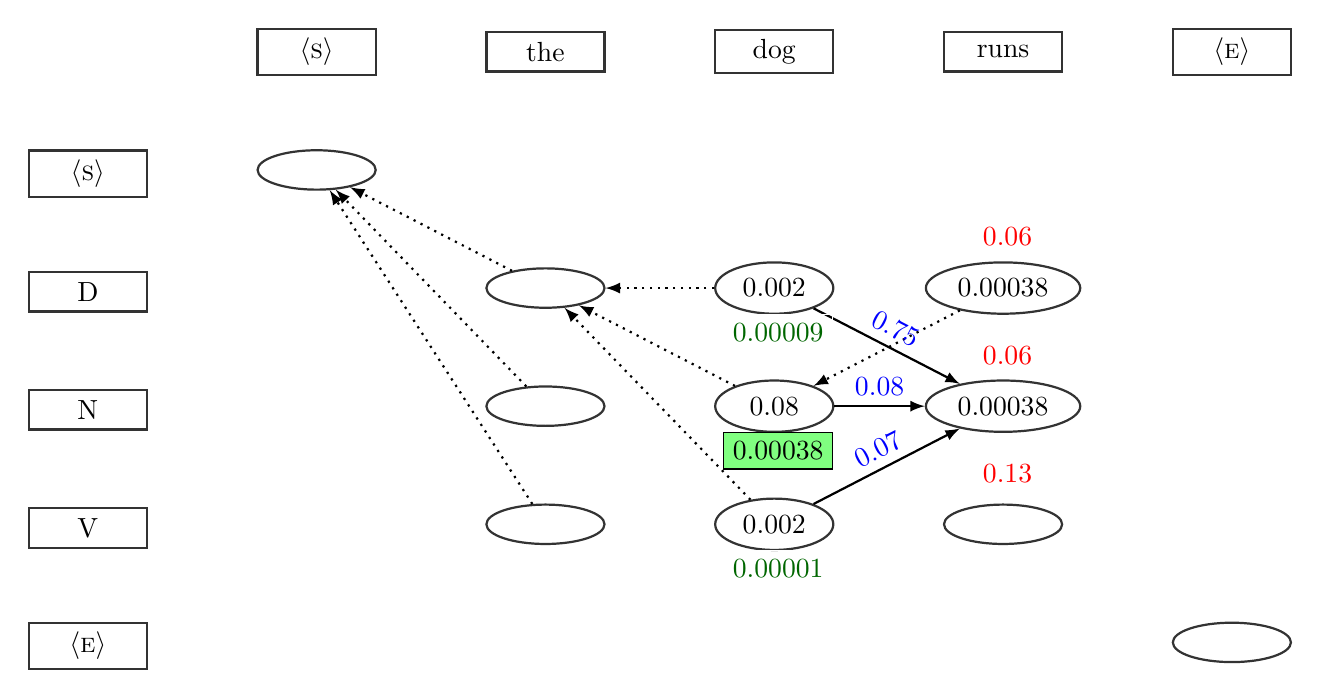
\begin{tikzpicture}
\tikzstyle{main}=[ellipse, thick, draw =black!80, node distance = 15mm, minimum height = 5mm, minimum width = 15mm]
\tikzstyle{rect}=[main, rectangle]
\tikzstyle{obsv}=[main, fill = black!10]
\tikzstyle{hidden}=[main, draw=white]
\tikzstyle{connect}=[-latex, thick]
\tikzstyle{box}=[rectangle, draw=black!100]

  
  \node[rect] (start) []                {\ngramstart};
  \node[rect] (D)     [below of =start] {D};
  \node[rect] (N)     [below of =D]     {N};
  \node[rect] (V)     [below of =N]     {V};
  \node[rect] (end)   [below of =V]     {\ngramend};

  \node[rect] (starttok) [right of =start,    xshift=40, yshift=44]   {\ngramstart};
  \node[rect] (the)      [right of =starttok, xshift=40]              {the};
  \node[rect] (dog)      [right of =the,      xshift=40]              {dog};
  \node[rect] (runs)     [right of =dog,      xshift=40]              {runs};
  \node[rect] (endtok)   [right of =runs,     xshift=40]              {\ngramend};

  \node[main] (startstart)  [below of =starttok]  {};

  \node[hidden] (startthe)  [below of =the]       {};
  \node[main] (Dthe)        [below of =startthe]  {};
  \node[main] (Nthe)        [below of =Dthe]      {};
  \node[main] (Vthe)        [below of =Nthe]      {};
  \node[hidden] (endthe)    [below of =Vthe]      {};

  \node[hidden] (startdog)  [below of =dog]       {};
  \node[main] (Ddog)        [below of =startdog]  {0.002};
  \node[main] (Ndog)        [below of =Ddog]      {0.08};
  \node[main] (Vdog)        [below of =Ndog]      {0.002};
  \node[hidden] (enddog)    [below of =Vdog]      {};

  \node[hidden] (startruns) [below of =runs]      {};
  \node[main] (Druns)       [below of =startruns] {0.00038};
  \node[draw, draw=white] at ([shift={(85:0.65)}]Druns) {\color{red}0.06};
  \node[main] (Nruns)       [below of =Druns]     {0.00038};
  \node[draw, draw=white] at ([shift={(85:0.65)}]Nruns) {\color{red}0.06};
  \node[main] (Vruns)       [below of =Nruns]     {};
  \node[draw, draw=white] at ([shift={(85:0.65)}]Vruns) {\color{red}0.13};
  \node[hidden] (endruns)   [below of =Vruns]     {};

  \node[hidden] (startend)  [below of =endtok]    {};
  \node[hidden] (Dend)      [below of =startend]  {};
  \node[hidden] (Nend)      [below of =Dend]      {};
  \node[hidden] (Vend)      [below of =Nend]      {};
  \node[main]   (endend)    [below of =Vend]      {};


  
  
  \path (Dthe) edge [connect, dotted] (startstart);
  \path (Nthe) edge [connect, dotted] (startstart);
  \path (Vthe) edge [connect, dotted] (startstart);
  \path (Ddog) edge [connect, dotted] (Dthe);
  \path (Ndog) edge [connect, dotted] (Dthe);
  \path (Vdog) edge [connect, dotted] (Dthe);
  \path (Druns) edge [connect, dotted] (Ndog);

  \path (Ddog) edge [connect] node [pos=0.5, above, blue, sloped] {0.75} (Nruns);
  \path (Ndog) edge [connect] node [pos=0.5, above, blue, sloped] {0.08} (Nruns);
  \path (Vdog) edge [connect] node [pos=0.5, above, blue, sloped] {0.07} (Nruns);
  
  \node[draw, draw=white] at ([shift={(95:-0.57)}]Ddog) {\color{black!60!green}0.00009};
  \node[draw, fill=white!50!green] at ([shift={(95:-0.57)}]Ndog) {0.00038};
  \node[draw, draw=white] at ([shift={(95:-0.57)}]Vdog) {\color{black!60!green}0.00001};


\end{tikzpicture}
\caption{Viterbi Algorithm: Calculate $v_3(N)$ and find the best path to it, which turns out to be the path ending with $t_2=N$}
\end{figure} 




\begin{figure}[p]
\centering
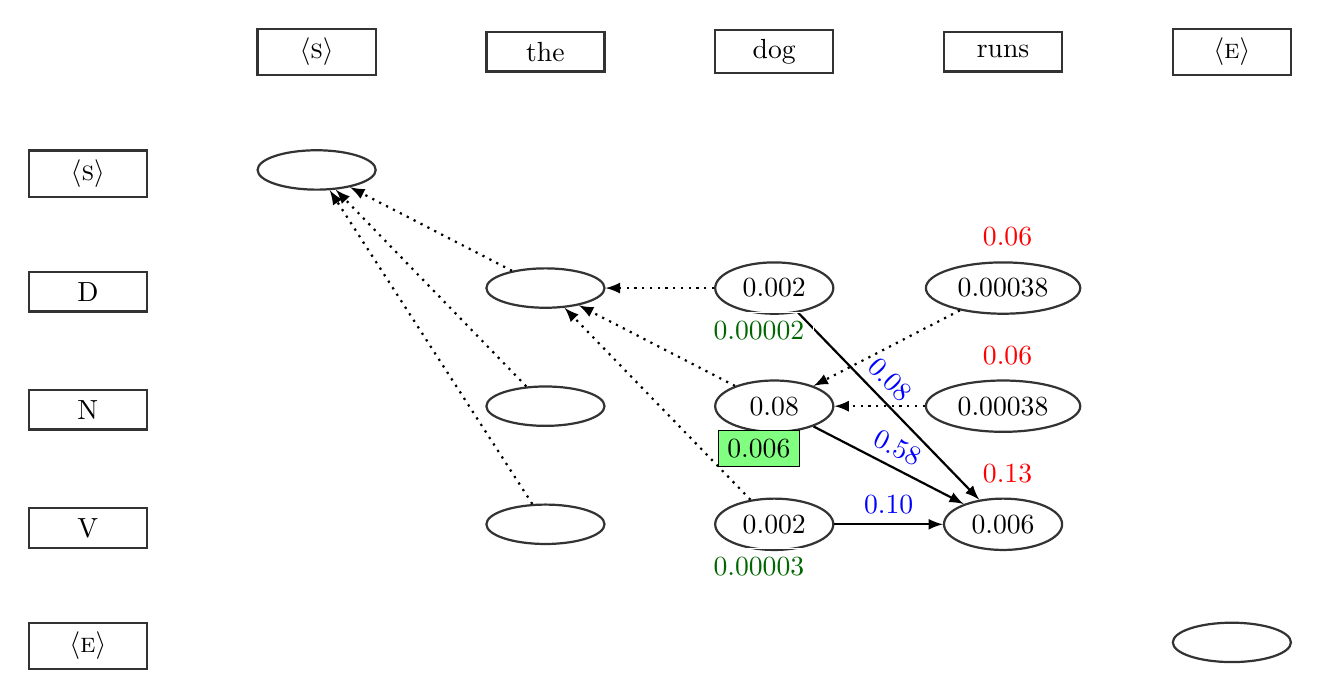
\begin{tikzpicture}
\tikzstyle{main}=[ellipse, thick, draw =black!80, node distance = 15mm, minimum height = 5mm, minimum width = 15mm]
\tikzstyle{rect}=[main, rectangle]
\tikzstyle{obsv}=[main, fill = black!10]
\tikzstyle{hidden}=[main, draw=white]
\tikzstyle{connect}=[-latex, thick]
\tikzstyle{box}=[rectangle, draw=black!100]

  
  \node[rect] (start) []                {\ngramstart};
  \node[rect] (D)     [below of =start] {D};
  \node[rect] (N)     [below of =D]     {N};
  \node[rect] (V)     [below of =N]     {V};
  \node[rect] (end)   [below of =V]     {\ngramend};

  \node[rect] (starttok) [right of =start,    xshift=40, yshift=44]   {\ngramstart};
  \node[rect] (the)      [right of =starttok, xshift=40]              {the};
  \node[rect] (dog)      [right of =the,      xshift=40]              {dog};
  \node[rect] (runs)     [right of =dog,      xshift=40]              {runs};
  \node[rect] (endtok)   [right of =runs,     xshift=40]              {\ngramend};

  \node[main] (startstart)  [below of =starttok]  {};

  \node[hidden] (startthe)  [below of =the]       {};
  \node[main] (Dthe)        [below of =startthe]  {};
  \node[main] (Nthe)        [below of =Dthe]      {};
  \node[main] (Vthe)        [below of =Nthe]      {};
  \node[hidden] (endthe)    [below of =Vthe]      {};

  \node[hidden] (startdog)  [below of =dog]       {};
  \node[main] (Ddog)        [below of =startdog]  {0.002};
  \node[main] (Ndog)        [below of =Ddog]      {0.08};
  \node[main] (Vdog)        [below of =Ndog]      {0.002};
  \node[hidden] (enddog)    [below of =Vdog]      {};

  \node[hidden] (startruns) [below of =runs]      {};
  \node[main] (Druns)       [below of =startruns] {0.00038};
  \node[draw, draw=white] at ([shift={(85:0.65)}]Druns) {\color{red}0.06};
  \node[main] (Nruns)       [below of =Druns]     {0.00038};
  \node[draw, draw=white] at ([shift={(85:0.65)}]Nruns) {\color{red}0.06};
  \node[main] (Vruns)       [below of =Nruns]     {0.006};
  \node[draw, draw=white] at ([shift={(85:0.65)}]Vruns) {\color{red}0.13};
  \node[hidden] (endruns)   [below of =Vruns]     {};

  \node[hidden] (startend)  [below of =endtok]    {};
  \node[hidden] (Dend)      [below of =startend]  {};
  \node[hidden] (Nend)      [below of =Dend]      {};
  \node[hidden] (Vend)      [below of =Nend]      {};
  \node[main]   (endend)    [below of =Vend]      {};


  
  \path (Dthe) edge [connect, dotted] (startstart);
  \path (Nthe) edge [connect, dotted] (startstart);
  \path (Vthe) edge [connect, dotted] (startstart);
  \path (Ddog) edge [connect, dotted] (Dthe);
  \path (Ndog) edge [connect, dotted] (Dthe);
  \path (Vdog) edge [connect, dotted] (Dthe);
  \path (Druns) edge [connect, dotted] (Ndog);
  \path (Nruns) edge [connect, dotted] (Ndog);

  \path (Ddog) edge [connect] node [pos=0.43, above, blue, sloped] {0.08} (Vruns);
  \path (Ndog) edge [connect] node [pos=0.5, above, blue, sloped] {0.58} (Vruns);
  \path (Vdog) edge [connect] node [pos=0.5, above, blue, sloped] {0.10} (Vruns);
  
  \node[draw, draw=white] at ([shift={(70:-0.57)}]Ddog) {\color{black!60!green}0.00002};
  \node[draw, fill=white!50!green] at ([shift={(70:-0.57)}]Ndog) {0.006};
  \node[draw, draw=white] at ([shift={(70:-0.57)}]Vdog) {\color{black!60!green}0.00003};
  

\end{tikzpicture}
\caption{Viterbi Algorithm: Calculate $v_3(V)$ and find the best path to it, which turns out to be the path ending with $t_2=N$}
\end{figure} 





\begin{figure}[p]
\centering
\begin{tikzpicture}
\tikzstyle{main}=[ellipse, thick, draw =black!80, node distance = 15mm, minimum height = 5mm, minimum width = 15mm]
\tikzstyle{rect}=[main, rectangle]
\tikzstyle{obsv}=[main, fill = black!10]
\tikzstyle{hidden}=[main, draw=white]
\tikzstyle{connect}=[-latex, thick]
\tikzstyle{box}=[rectangle, draw=black!100]

  
  \node[rect] (start) []                {\ngramstart};
  \node[rect] (D)     [below of =start] {D};
  \node[rect] (N)     [below of =D]     {N};
  \node[rect] (V)     [below of =N]     {V};
  \node[rect] (end)   [below of =V]     {\ngramend};

  \node[rect] (starttok) [right of =start,    xshift=40, yshift=44]   {\ngramstart};
  \node[rect] (the)      [right of =starttok, xshift=40]              {the};
  \node[rect] (dog)      [right of =the,      xshift=40]              {dog};
  \node[rect] (runs)     [right of =dog,      xshift=40]              {runs};
  \node[rect] (endtok)   [right of =runs,     xshift=40]              {\ngramend};

  \node[main] (startstart)  [below of =starttok]  {};

  \node[hidden] (startthe)  [below of =the]       {};
  \node[main] (Dthe)        [below of =startthe]  {};
  \node[main] (Nthe)        [below of =Dthe]      {};
  \node[main] (Vthe)        [below of =Nthe]      {};
  \node[hidden] (endthe)    [below of =Vthe]      {};

  \node[hidden] (startdog)  [below of =dog]       {};
  \node[main] (Ddog)        [below of =startdog]  {};
  \node[main] (Ndog)        [below of =Ddog]      {};
  \node[main] (Vdog)        [below of =Ndog]      {};
  \node[hidden] (enddog)    [below of =Vdog]      {};

  \node[hidden] (startruns) [below of =runs]      {};
  \node[main] (Druns)       [below of =startruns] {0.00038};
  \node[draw, draw=white] at ([shift={(55:-0.67)}]Druns) {\color{black!60!green}0.00003};
  \node[main] (Nruns)       [below of =Druns]     {0.00038};
  \node[draw, draw=white] at ([shift={(55:-0.67)}]Nruns) {\color{black!60!green}0.0001};
  \node[main] (Vruns)       [below of =Nruns]     {0.006};
  \node[draw, fill=white!50!green] at ([shift={(55:-0.67)}]Vruns) {\color{black!60!green}0.003};
  \node[hidden] (endruns)   [below of =Vruns]     {};

  \node[hidden] (startend)  [below of =endtok]    {};
  \node[hidden] (Dend)      [below of =startend]  {};
  \node[hidden] (Nend)      [below of =Dend]      {};
  \node[hidden] (Vend)      [below of =Nend]      {};
  \node[draw, draw=white] at ([shift={(85:0.65)}]endend) {\color{red}1.0};
  \node[main]   (endend)    [below of =Vend]      {};


  \path (Dthe) edge [connect, dotted] (startstart);
  \path (Nthe) edge [connect, dotted] (startstart);
  \path (Vthe) edge [connect, dotted] (startstart);
  \path (Ddog) edge [connect, dotted] (Dthe);
  \path (Ndog) edge [connect, dotted] (Dthe);
  \path (Vdog) edge [connect, dotted] (Dthe);
  \path (Druns) edge [connect, dotted] (Ndog);
  \path (Nruns) edge [connect, dotted] (Ndog);
  \path (Vruns) edge [connect, dotted] (Ndog);
  
  \path (Druns) edge [connect] node [pos=0.35, above, blue, sloped] {0.08} (endend);
  \path (Nruns) edge [connect] node [pos=0.25, above, blue, sloped] {0.25} (endend);
  \path (Vruns) edge [connect] node [pos=0.25, above, blue, sloped] {0.50} (endend);
  

\end{tikzpicture}
\caption{Viterbi Algorithm: Calculate $v_4(\ngramend)$ and find the best path to it, which turns out to be the path ending with $t_3=V$}
\end{figure} 





\begin{figure}[p]
\centering
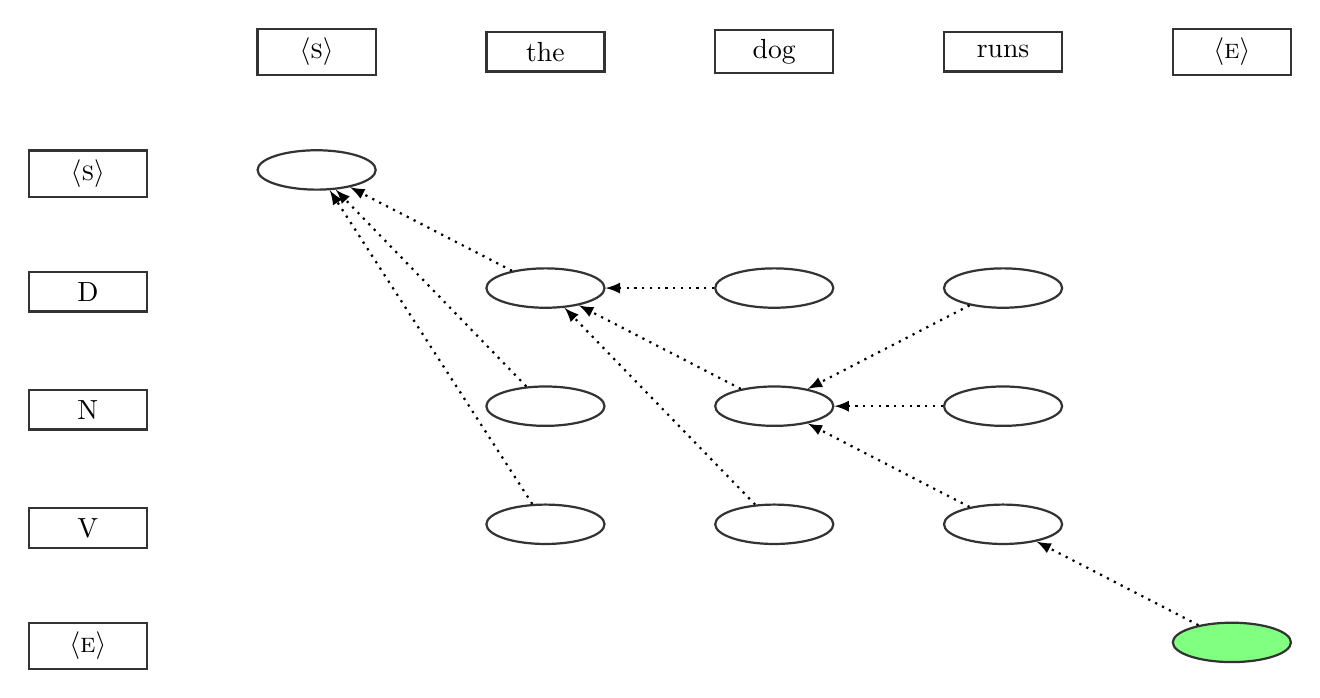
\begin{tikzpicture}
\tikzstyle{main}=[ellipse, thick, draw =black!80, node distance = 15mm, minimum height = 5mm, minimum width = 15mm]
\tikzstyle{rect}=[main, rectangle]
\tikzstyle{obsv}=[main, fill = black!10]
\tikzstyle{hidden}=[main, draw=white]
\tikzstyle{connect}=[-latex, thick]
\tikzstyle{box}=[rectangle, draw=black!100]

  
  \node[rect] (start) []                {\ngramstart};
  \node[rect] (D)     [below of =start] {D};
  \node[rect] (N)     [below of =D]     {N};
  \node[rect] (V)     [below of =N]     {V};
  \node[rect] (end)   [below of =V]     {\ngramend};

  \node[rect] (starttok) [right of =start,    xshift=40, yshift=44]   {\ngramstart};
  \node[rect] (the)      [right of =starttok, xshift=40]              {the};
  \node[rect] (dog)      [right of =the,      xshift=40]              {dog};
  \node[rect] (runs)     [right of =dog,      xshift=40]              {runs};
  \node[rect] (endtok)   [right of =runs,     xshift=40]              {\ngramend};

  \node[main] (startstart)  [below of =starttok]  {};

  \node[hidden] (startthe)  [below of =the]       {};
  \node[main] (Dthe)        [below of =startthe]  {};
  \node[main] (Nthe)        [below of =Dthe]      {};
  \node[main] (Vthe)        [below of =Nthe]      {};
  \node[hidden] (endthe)    [below of =Vthe]      {};

  \node[hidden] (startdog)  [below of =dog]       {};
  \node[main] (Ddog)        [below of =startdog]  {};
  \node[main] (Ndog)        [below of =Ddog]      {};
  \node[main] (Vdog)        [below of =Ndog]      {};
  \node[hidden] (enddog)    [below of =Vdog]      {};

  \node[hidden] (startruns) [below of =runs]      {};
  \node[main] (Druns)       [below of =startruns] {};
  \node[main] (Nruns)       [below of =Druns]     {};
  \node[main] (Vruns)       [below of =Nruns]     {};
  \node[hidden] (endruns)   [below of =Vruns]     {};

  \node[hidden] (startend)  [below of =endtok]    {};
  \node[hidden] (Dend)      [below of =startend]  {};
  \node[hidden] (Nend)      [below of =Dend]      {};
  \node[hidden] (Vend)      [below of =Nend]      {};
  \node[main, fill=white!50!green]   (endend)    [below of =Vend]      {};


  \path (Dthe) edge [connect, dotted] (startstart);
  \path (Nthe) edge [connect, dotted] (startstart);
  \path (Vthe) edge [connect, dotted] (startstart);
  \path (Ddog) edge [connect, dotted] (Dthe);
  \path (Ndog) edge [connect, dotted] (Dthe);
  \path (Vdog) edge [connect, dotted] (Dthe);
  \path (Druns) edge [connect, dotted] (Ndog);
  \path (Nruns) edge [connect, dotted] (Ndog);
  \path (Vruns) edge [connect, dotted] (Ndog);
  \path (endend) edge [connect, dotted] (Vruns);
  

\end{tikzpicture}
\caption{Viterbi Algorithm: The tag for \ngramend\ is always \ngramend, so we can always start by selecting that tag.}
\end{figure} 




\begin{figure}[p]
\centering
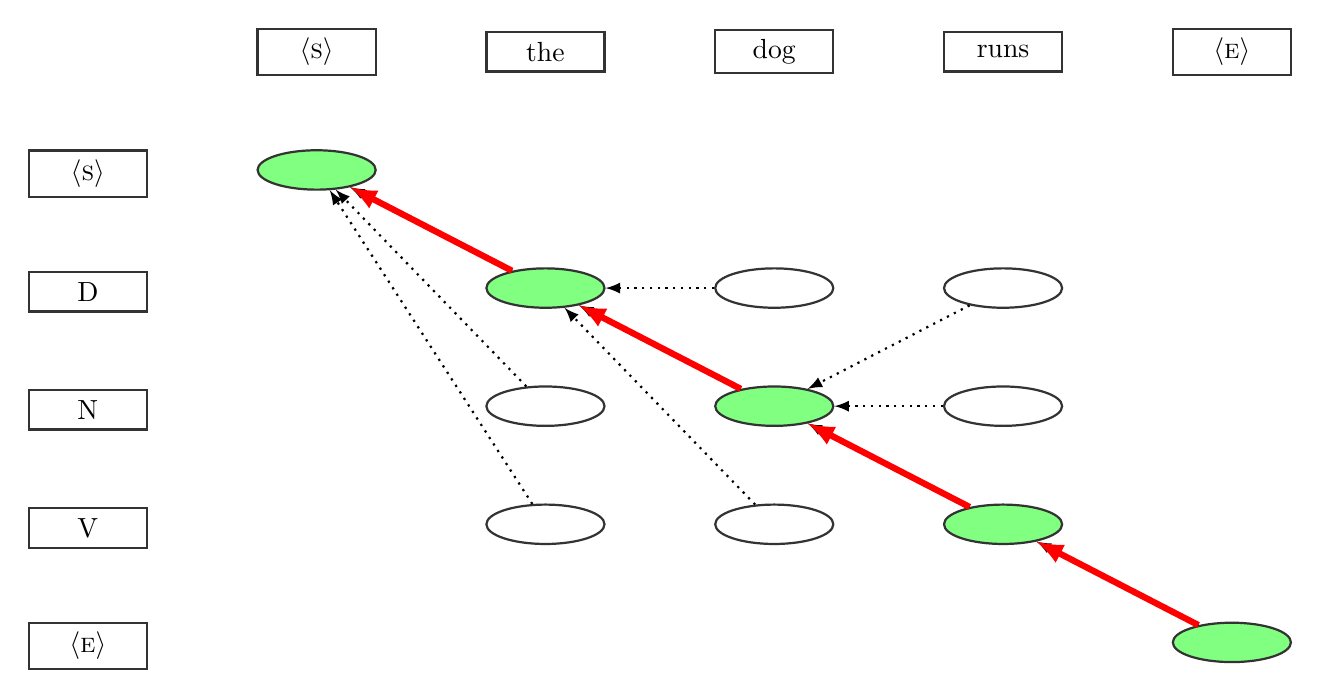
\begin{tikzpicture}
\tikzstyle{main}=[ellipse, thick, draw =black!80, node distance = 15mm, minimum height = 5mm, minimum width = 15mm]
\tikzstyle{rect}=[main, rectangle]
\tikzstyle{obsv}=[main, fill = black!10]
\tikzstyle{hidden}=[main, draw=white]
\tikzstyle{connect}=[-latex, thick]
\tikzstyle{box}=[rectangle, draw=black!100]

  
  \node[rect] (start) []                {\ngramstart};
  \node[rect] (D)     [below of =start] {D};
  \node[rect] (N)     [below of =D]     {N};
  \node[rect] (V)     [below of =N]     {V};
  \node[rect] (end)   [below of =V]     {\ngramend};

  \node[rect] (starttok) [right of =start,    xshift=40, yshift=44]   {\ngramstart};
  \node[rect] (the)      [right of =starttok, xshift=40]              {the};
  \node[rect] (dog)      [right of =the,      xshift=40]              {dog};
  \node[rect] (runs)     [right of =dog,      xshift=40]              {runs};
  \node[rect] (endtok)   [right of =runs,     xshift=40]              {\ngramend};

  \node[main, fill=white!50!green] (startstart)  [below of =starttok]  {};

  \node[hidden] (startthe)  [below of =the]       {};
  \node[main, fill=white!50!green] (Dthe)        [below of =startthe]  {};
  \node[main] (Nthe)        [below of =Dthe]      {};
  \node[main] (Vthe)        [below of =Nthe]      {};
  \node[hidden] (endthe)    [below of =Vthe]      {};

  \node[hidden] (startdog)  [below of =dog]       {};
  \node[main] (Ddog)        [below of =startdog]  {};
  \node[main, fill=white!50!green] (Ndog)        [below of =Ddog]      {};
  \node[main] (Vdog)        [below of =Ndog]      {};
  \node[hidden] (enddog)    [below of =Vdog]      {};

  \node[hidden] (startruns) [below of =runs]      {};
  \node[main] (Druns)       [below of =startruns] {};
  \node[main] (Nruns)       [below of =Druns]     {};
  \node[main, fill=white!50!green] (Vruns)       [below of =Nruns]     {};
  \node[hidden] (endruns)   [below of =Vruns]     {};

  \node[hidden] (startend)  [below of =endtok]    {};
  \node[hidden] (Dend)      [below of =startend]  {};
  \node[hidden] (Nend)      [below of =Dend]      {};
  \node[hidden] (Vend)      [below of =Nend]      {};
  \node[main, fill=white!50!green]   (endend)    [below of =Vend]      {};



  \path (Dthe) edge [connect, dotted] (startstart);
  \path (Nthe) edge [connect, dotted] (startstart);
  \path (Vthe) edge [connect, dotted] (startstart);
  \path (Ddog) edge [connect, dotted] (Dthe);
  \path (Ndog) edge [connect, dotted] (Dthe);
  \path (Vdog) edge [connect, dotted] (Dthe);
  \path (Druns) edge [connect, dotted] (Ndog);
  \path (Nruns) edge [connect, dotted] (Ndog);
  \path (Vruns) edge [connect, dotted] (Ndog);
  \path (endend) edge [connect, dotted] (Vruns);
  
  \path (Dthe) edge [connect, line width=0.8mm, red] (startstart);
  \path (Ndog) edge [connect, line width=0.8mm, red] (Dthe);
  \path (Vruns) edge [connect, line width=0.8mm, red] (Ndog);  
  \path (endend) edge [connect, line width=0.8mm, red] (Vruns);
  

\end{tikzpicture}
\caption{Viterbi Algorithm: For each tag $t_{i+1}$, we examine the backpointer that indicates the way to the best path to $t_{i+1}$, and choose $t_i$ accordingly.}
\end{figure} 





% \begin{align*}

% \end{align*}


\section{Tag Dictionary}

\begin{itemize}
  \item Mapping from words to potential tags
  \item Get from train, assume it works on test
  \item Unseen words usually assumed to be any possible tag.  Could, instead, assume only open-class tags.
  \item Prune low-probability tags.
\end{itemize}


\section{Semi-Supervised Learning: The Forward-Backward Algorithm}

\begin{itemize}
  \item Given some unlabeled text, and a set of labels, learn the best set of parameters for an HMM tagger.
  \item Usually needs a tag dictionary to constrain the search space.
  \item Similar to Viterbi, but instead of finding the max-probability path, we estimate the probability of each tag for each token.
  \item forward$_i(k)$: probability of begin in state $k$ after seeing the first $i$ words (by summing over all paths leading to $k$)
  \item backward$_i(k)$: probability of seeing sequence of tags from $i$+1 to $N$, given that $t_i=k$
\end{itemize}
\begin{align*}
  forward_i(k) %&= p(t_i=k \mid w_{1:i}) \\
               %&= p(w_i \mid k) \cdot \sum_{k' \in T} p(k \mid k') \cdot p(t_{i-1}=k' \mid w_{1:i-1}) \\
               &= p(w_i \mid k) \cdot \sum_{k' \in T} p(k \mid k') \cdot forward_{i-1}(k') \\\\
  backward_i(k) %&= p(t_i=k' \mid t_{i+1}, w_{1:N}) \\
                %&= \sum_{k \in T} p(k \mid k') \cdot p(w_{i+1} \mid k) \cdot p(t_{i+1}=k \mid w_{1:i+1}) \\
                &= \sum_{k' \in T} p(k' \mid k) \cdot p(w_{i+1} \mid k') \cdot backward_{i+1}(k')
\end{align*}

expected transitions from $t_i=k_1$ to $t_{i+1}=k_2$: 
\[
  \frac{forward_i(k_1) \cdot p(k_2 \mid k_1) \cdot p(w_{i+1} \mid k_2) \cdot backward_{i+1}(k_2)}
       {p(w_{1:N})}
\]

expected emissions of $w_i$ when $t_i=k$
\[
  \frac{forward_i(k) \cdot backward_i(k)}
       {p(w_{1:N})}
\]

Re-estimating transitions:
\begin{align*}
  p(t_2 \mid t_1) &= \frac{\text{expected number of transitions from $t_1$ to $t_2$}}
                          {\text{expected number of transitions from $t_1$}}
\end{align*}

Re-estimating emissions:
\begin{align*}
  p(w \mid t) &= \frac{\text{expected number of times word $w$ occurs with tag $t$}}
                      {\text{expected number of times tag $t$ occurs}}
\end{align*}

The Forward-Backward Algorithm (Expectation-Maximization):

\begin{itemize}
  \item E Step: Use $forward$ and $backward$ to compute the expected transition and emission counts
  \item M Step: Re-estimate transition and emission distributions from expected counts
\end{itemize}


\end{document}

